% !TEX root = main.tex

\section{语言模型}
语言模型主要包括统计语言模型和神经语言模型。

\subsection{统计语言模型}
考虑语句的先验概率
\[p(s)=\prod_{i=1}^{m}p(w_i\mid w_1\cdots w_{i-1}),\;p(w_1\mid w_0)=p(w_1)\]
其中$w_i$可以是字、词、短语等,称为\textbf{统计基元},通常用\underline{词}代之。

为减少历史基元的个数,将$w_1w_2\cdots w_{i-1}$映射到等价类$S(w_1w_2\cdots w_{i-1})$,使等价类的数目远小于原来不同历史基元的数目,则有
\[p(w_i\mid w_1\cdots w_{i-1})=p(w_i\mid S(w_1\cdots w_{i-1}))\]

n元文法(n-gram)模型
\begin{itemize}
	\item 当$n=1$时,出现在第$i$位上的基元$w_i$独立于历史,1元文法也被uni-gram或monogram
	\item $n=2$时,2-gram(bi-gram)称为1阶马尔可夫链
	\item $n=3$时,3-gram(tri-gram)称为2阶马尔可夫链,以此类推
\end{itemize}
实际操作加上句首\verb'<BOS>'和句尾标记\verb'<EOS>'。
\begin{figure}[H]
\centering
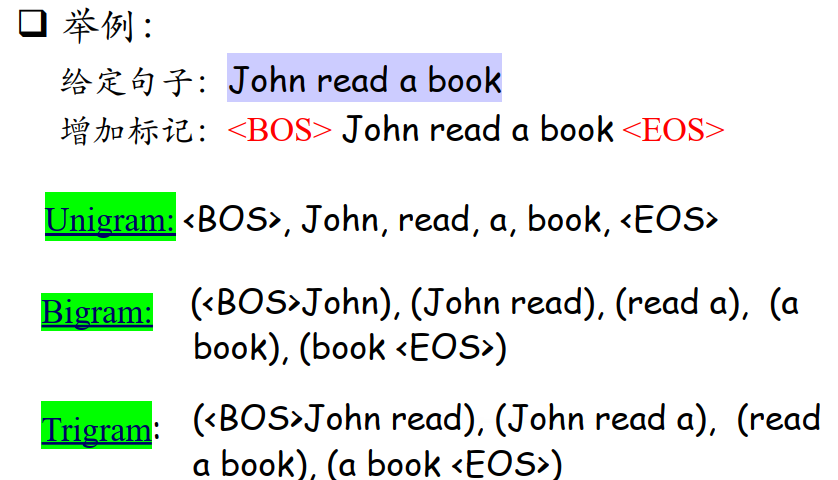
\includegraphics[width=0.6\linewidth]{fig/n-gram.png}
\end{figure}

应用:
\begin{itemize}
	\item 音字转换问题:给定拼音转为汉字串
	\item 汉语分词问题
\end{itemize}

对于n-gram,由最大似然估计求得
\[p(w_i\mid w_{i-n+1}^{i-1})=f(w_i\mid w_{i-n+1}^{i-1})=\frac{c(w_{i-1+1})}{\sum_{w_i}c(w_{i-n+1}^i)}\]
其中$\sum_{w_i}c(w_{i-n+1}^i)$是历史串$w_{i-n+1}^{i-1}$在给定语料中出现的次数,即$c(w_{i-n+1}^{i-1})$。

\begin{definition}[困惑度(perplexity)]
假定测试语料$T$由$L$个句子$(t_1,\ldots,t_L)$构成,则整个测试集的概率为
\[p(T)=\prod_{i=1}^Lp(t_i)\]
\end{definition}

为避免数据匮乏/稀疏导致的零概率问题,需要做数据平滑:调整最大似然估计的概率值,使零概率增值,使非零概率下调,消除零概率,改进模型的整体正确率。
基本目标是测试样本语言模型的\textbf{困惑度越小越好},基本约束是
\[\sum_{w_i}p(w_i\mid w_1,w_2,\ldots,w_{i-1})=1\]
\begin{itemize}
	\item 加一法:
	\[p(w_i\mid w_{i-1}=\frac{1+c(w_{i-1}w_i)}{|V|+\sum_{w_i}c(w_{i-1}w_i)}\]
	\item 减值法/折扣法:将剩余概率量分配给未见概率
	\begin{itemize}
		\item Good-Turing估计
		\item 绝对减值法:从每个计数$r$中减去相同的量,剩余概率量由未见事件均分
		\[p_r=\begin{cases}
		\frac{r-b}{N} & r>0\\
		\frac{b(R-n_0)}{Nn_0} & r=0
		\end{cases}\]
		其中$n_0$为样本中未出现的事件数目,$b\leq 1$为减去的常量,$b(R-n_0)/N$是由于减值而产生的剩余概率量
	\end{itemize}
\end{itemize}

\subsection{神经语言模型}
对于固定窗口大小的神经网络显然是不适用的,需要采用一种能够处理任意长度输入的架构,即循环神经网络(RNN),不同神经元共享相同的参数。
\begin{figure}[H]
\centering
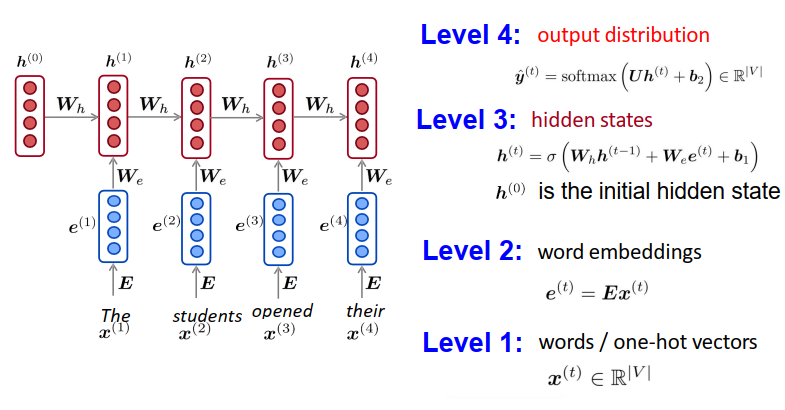
\includegraphics[width=0.6\linewidth]{fig/RNN.png}
\end{figure}

RNN的优点:
\begin{itemize}
	\item 能够处理任意长度输入
	\item $t$时刻可以访问之前任意时刻的信息
	\item 对于较长输入,模型大小不变
	\item 权重共享
\end{itemize}

不足:循环计算过程慢,难以访问到距当前时刻较远的信息。